\documentclass[journal,12pt,twocolumn]{IEEEtran}
\usepackage{setspace}
\usepackage{gensymb}
\singlespacing
\usepackage[cmex10]{amsmath}
\usepackage{amsthm}
\usepackage{mathrsfs}
\usepackage{txfonts}
\usepackage{stfloats}
\usepackage{bm}
\usepackage{cite}
\usepackage{cases}
\usepackage{subfig}
\usepackage{longtable}
\usepackage{multirow}
\usepackage{enumitem}
\usepackage{mathtools}
\usepackage{steinmetz}
\usepackage{tikz}
\usepackage{circuitikz}
\usepackage{verbatim}
\usepackage{tfrupee}
\usepackage[breaklinks=true]{hyperref}
\usepackage{graphicx}
\usepackage{tkz-euclide}
\usetikzlibrary{calc,math}
\usepackage{listings}
\usepackage{color}                                            %%
\usepackage{array}                                            %%
\usepackage{longtable}                                        %%
\usepackage{calc}                                             %%
\usepackage{multirow}                                         %%
\usepackage{hhline}                                           %%
\usepackage{ifthen}                                           %%
\usepackage{lscape}     
\usepackage{multicol}
\usepackage{chngcntr}
\DeclareMathOperator*{\Res}{Res}
\renewcommand\thesection{\arabic{section}}
\renewcommand\thesubsection{\thesection.\arabic{subsection}}
\renewcommand\thesubsubsection{\thesubsection.\arabic{subsubsection}}
\renewcommand\thesectiondis{\arabic{section}}
\renewcommand\thesubsectiondis{\thesectiondis.\arabic{subsection}}
\renewcommand\thesubsubsectiondis{\thesubsectiondis.\arabic{subsubsection}}
\hyphenation{op-tical net-works semi-conduc-tor}
\def\inputGnumericTable{}                                 %%

\lstset{
%language=C,
frame=single, 
breaklines=true,
columns=fullflexible
}
\begin{document}
\newtheorem{theorem}{Theorem}[section]
\newtheorem{problem}{Problem}
\newtheorem{proposition}{Proposition}[section]
\newtheorem{lemma}{Lemma}[section]
\newtheorem{corollary}[theorem]{Corollary}
\newtheorem{example}{Example}[section]
\newtheorem{definition}[problem]{Definition}
\newcommand{\BEQA}{\begin{eqnarray}}
\newcommand{\EEQA}{\end{eqnarray}}
\newcommand{\define}{\stackrel{\triangle}{=}}
\bibliographystyle{IEEEtran}
\raggedbottom
\setlength{\parindent}{0pt}
\providecommand{\mbf}{\mathbf}
\providecommand{\pr}[1]{\ensuremath{\Pr\left(#1\right)}}
\providecommand{\qfunc}[1]{\ensuremath{Q\left(#1\right)}}
\providecommand{\sbrak}[1]{\ensuremath{{}\left[#1\right]}}
\providecommand{\lsbrak}[1]{\ensuremath{{}\left[#1\right.}}
\providecommand{\rsbrak}[1]{\ensuremath{{}\left.#1\right]}}
\providecommand{\brak}[1]{\ensuremath{\left(#1\right)}}
\providecommand{\lbrak}[1]{\ensuremath{\left(#1\right.}}
\providecommand{\rbrak}[1]{\ensuremath{\left.#1\right)}}
\providecommand{\cbrak}[1]{\ensuremath{\left\{#1\right\}}}
\providecommand{\lcbrak}[1]{\ensuremath{\left\{#1\right.}}
\providecommand{\rcbrak}[1]{\ensuremath{\left.#1\right\}}}
\theoremstyle{remark}
\newtheorem{rem}{Remark}
\newcommand{\sgn}{\mathop{\mathrm{sgn}}}
%\providecommand{\abs}[1]{\left\vert#1\right\vert}
\providecommand{\res}[1]{\Res\displaylimits_{#1}} 
\providecommand{\norm}[1]{$\left\lVert#1\right\rVert$}
%\providecommand{\norm}[1]{\lVert#1\rVert}
\providecommand{\mtx}[1]{\mathbf{#1}}
\providecommand{\mean}[1]{E$\left[ #1 \right]$}
\providecommand{\fourier}{\overset{\mathcal{F}}{ \rightleftharpoons}}
%\providecommand{\hilbert}{\overset{\mathcal{H}}{ \rightleftharpoons}}
\providecommand{\system}{\overset{\mathcal{H}}{ \longleftrightarrow}}
%\newcommand{\solution}[2]{\textbf{Solution:}{#1}}
\newcommand{\solution}{\noindent \textbf{Solution: }}
\newcommand{\cosec}{\,\text{cosec}\,}
\providecommand{\dec}[2]{\ensuremath{\overset{#1}{\underset{#2}{\gtrless}}}}
\newcommand{\myvec}[1]{\ensuremath{\begin{pmatrix}#1\end{pmatrix}}}
\newcommand{\mydet}[1]{\ensuremath{\begin{vmatrix}#1\end{vmatrix}}}
\numberwithin{equation}{subsection}
\makeatletter
\@addtoreset{figure}{problem}
\makeatother
\let\StandardTheFigure\thefigure
\let\vec\mathbf
\renewcommand{\thefigure}{\theproblem}
\def\putbox#1#2#3{\makebox[0in][l]{\makebox[#1][l]{}\raisebox{\baselineskip}[0in][0in]{\raisebox{#2}[0in][0in]{#3}}}}
\def\rightbox#1{\makebox[0in][r]{#1}}
\def\centbox#1{\makebox[0in]{#1}}
\def\topbox#1{\raisebox{-\baselineskip}[0in][0in]{#1}}
\def\midbox#1{\raisebox{-0.5\baselineskip}[0in][0in]{#1}}
\vspace{3cm}
\title{EE3025-Assignment 1}
\author{Vamshika K - EE17BTECH11045}
\maketitle
\newpage
\bigskip
\renewcommand{\thefigure}{\theenumi}
\renewcommand{\thetable}{\theenumi}
Download all python codes from 
\begin{lstlisting}
https://github.com/vamshikak/EE3025/tree/main/Assignment_1/codes
\end{lstlisting}
%
and latex-tikz codes from 
%
\begin{lstlisting}
https://github.com/vamshikak/EE3025/tree/main/Assignment_1
\end{lstlisting}
\section{Problem}
5.3 The system h(n) is said to be stable if 
\begin{align}
\sum_{n=-\infty}^{\infty} \abs{|h(n)|} < \infty
\end{align} 
Is the system defined by (3.2) stable for impulse response in (5.1)?
\section{Solution}
\textbf{For the given system}
\begin{align}
    y(n)+\frac{1}{2}y(n-1) = x(n)+x(n-2) \\
    y(n)=0 \text{ for }n<0
\end{align}
On applying Z-transform on both sides, we get
\begin{align}
    Y(z) + \frac{1}{2}z^{-1}Y(z)=X(z) + z^{-2}X(z)\\
    Y(z)=\frac{1+z^{-2}}{1+\frac{1}{2}z^{-1}}X(z)\\
 \frac{Y(z)}{X(z)}=\frac{1+z^{-2}}{1+\frac{1}{2}z^{-1}}
\end{align}
Relation between z-transforms of input, output and impulse response is as follows
\begin{align}
    H(z) = \frac{Y(z)}{X(z)}
\end{align}
Hence 
\begin{align}
H(z)=\frac{1+z^{-2}}{1+\frac{1}{2}z^{-1}}
    =\frac{1}{1+\frac{1}{2}z^{-1}} + \frac{z^{-2}}{1+\frac{1}{2}z^{-1}}
\end{align}
Now, applying inverse Z-transform on both sides
\begin{align}
h(n)=\sbrak{\frac{-1}{2}}^nu(n) + \sbrak{\frac{-1}{2}}^{n-2}u(n-2)
\end{align}

\textbf {Checking for stability:}
We check if the system is stable using \textbf{BIBO stability condition} as follows
\begin{align}
    |x(n)|\leq B_x<\infty \implies |y(n)| \leq B_y<\infty
\end{align}
For every bounded input (x(n)) output (y(n)) of the system is bounded.

We know that in time domain, 
\begin{align}
    y(n)=\sum_{-\infty}^{\infty}h(k)x(n-k)
\end{align}
After applying mod on both sides,
\begin{align}
    |y(n)|=|\sum_{-\infty}^{\infty}h(k)x(n-k)|
\end{align}
From 2.0.9 lets suppose x(n) is bounded by Bx, then
\begin{align}
      |y(n)| \leq |\sum_{-\infty}^{\infty}h(k) B_x|\\
    |y(n)| \leq B_x|\sum_{-\infty}^{\infty}h(k)|
\end{align}
Since $|y(n)| < \infty$ for BIBO stability condition to hold for bounded input and holds only if
\begin{align}
    |\sum_{-\infty}^{\infty}h(k)| < \infty
\end{align}
Hence, impulse response of system in time domain must be absolutely sumable for it to be BIBO stable.

Now, checking if system is BIBO stable for 2.0.8\
\begin{align}
    \sum_{n=-\infty}^{\infty}|\abs{\sbrak{\frac{-1}{2}}^nu(n) + \sbrak{\frac{-1}{2}}^{n-2}u(n-2)}| < \infty \\
     \sum_{n=-\infty}^{\infty}|\abs{\sbrak{\frac{1}{2}}^nu(n) + \sbrak{\frac{1}{2}}^{n-2}u(n-2)}| < \infty \\
     2\sum_{n=-\infty}^{\infty}|\abs{\sbrak{\frac{1}{2}}^nu(n)}| < \infty \\
     2\sbrak{\frac{1}{1-\frac{1}{2}}} < \infty \\
    4 < \infty
\end{align}
Our system is BIBO stable since the condition hold.\\

\textbf{Example Input:}
Our system,
\begin{align}
    y(n)+\frac{1}{2}y(n-1) = x(n)+x(n-2) \\
    y(n)=0 \text{ for }n<0
\end{align}
Lets consider the input to be
\begin{align}
    x(n)= [1.0,2.0,1.0,4.0,3.0,3.0]
\end{align}

\renewcommand{\thefigure}{A\arabic{figure}}

\setcounter{figure}{0}
\begin{figure}[htp]
   \centering Figure
    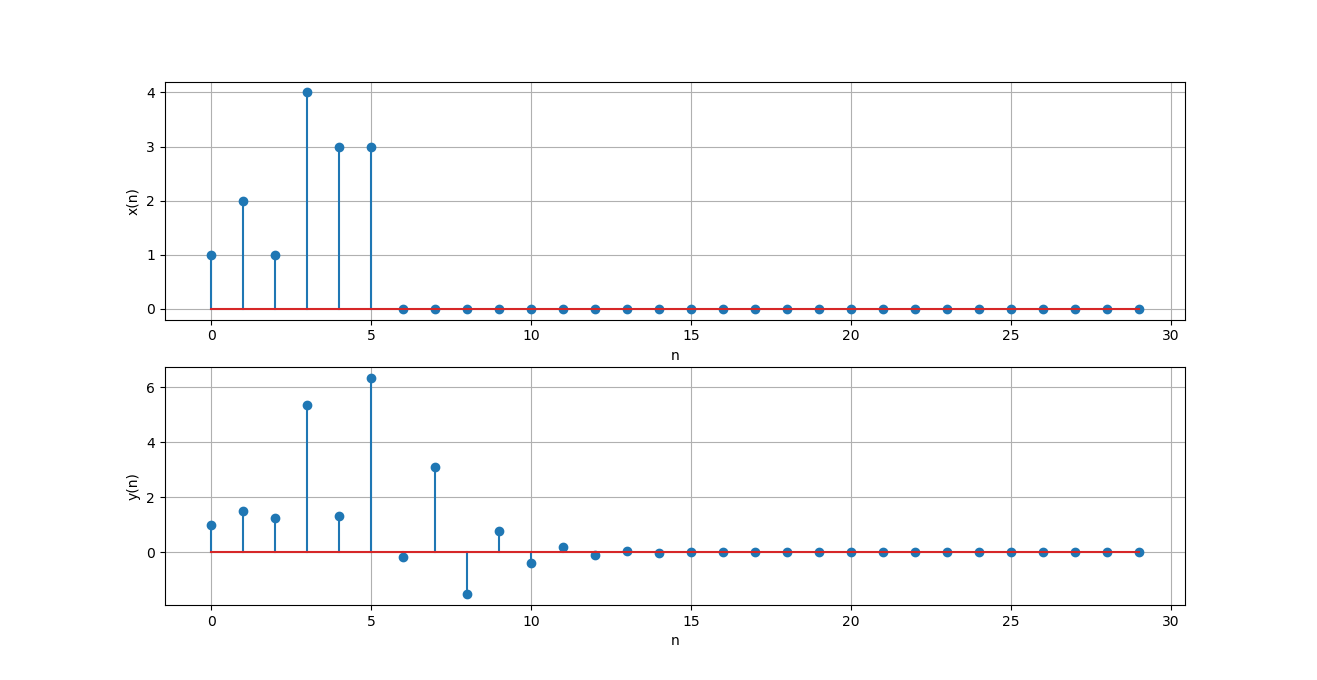
\includegraphics[width=9cm]{Figure_1.png}
    \caption{Input signal x(n) and Output signal y(n)}
\end{figure}

We know that for our input signal $B_x=4$ and after calculating for output we get $B_y=6.34375$ as shown in Fig. A1. Since both input and output are less then infinity(bounded), BIBO stability holds.\\

\textbf{Stability by Region Of Convergence(ROC):}
\textbf{Method 1:}
For a system to be stable, its ROC must include unit circle. By solving 2.0.7 for poles and zeros we get as follows.
\begin{align}
    Poles = 0 , -\frac{1}{2} \\
    Zeros = +1j, -1j
\end{align}
After plotting it can be seen that ROC includes unit circle and hence stable.

\textbf{Method 2:}
We know that
\begin{align}
    \sum_{n=-\infty}^{\infty} |\abs{h(n)}|  &< \infty 
\end{align}
Considering h(n) is absolutely summable
\begin{align}
    \sum_{n=-\infty}^{\infty}\abs{|h(n)z^{-n}|}_{|\abs{z}|=1}&<\infty 
\end{align}
By triangle inequality, following holds
\begin{align}
   \implies \abs{|\sum_{n=-\infty}^{\infty}h(n)z^{-n}|}_\abs{|z|=1}<\sum_{n=-\infty}^{\infty}\abs{|h(n)z^{-n}|}_{\abs{|z|}=1}
\end{align}
by substituting 2.0.27 in 2.0.26
\begin{align}
   \abs{|H(z)|}_{\abs{|z|}=1}&<\infty 
\end{align}
Hence, ROC includes unit circle as shown in Fig. A2. By both the above methods it can be said that system is stability 
\begin{figure}[htp]
    \centering Figure
    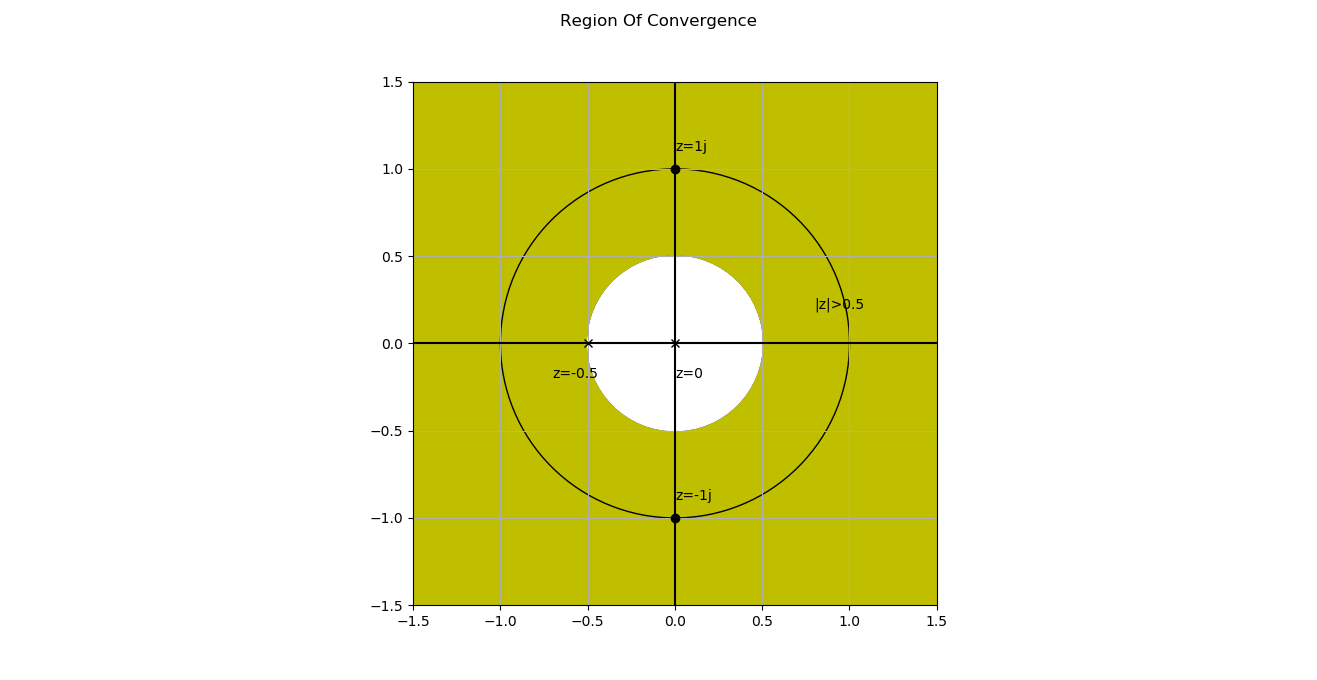
\includegraphics[width=10cm]{Figure_2.png}
    \caption{Plot for Pole-Zero}
\end{figure}\\
\end{document}